\documentclass[10pt, a4paper,xcolor=table]{beamer}

\usetheme{Berkeley}
\usepackage{graphicx}
\graphicspath{ {./images/} }
\usecolortheme{sidebartab}

\begin{document}
	\setbeamertemplate{sidebar left}{}
	\title{Progress Presentation - I}
	\subtitle{e-Yantra Summer Intership - 2017 \\ Vegetable Identification \\ using Transfer Learning}
	\author{Sanket Shanbhag\\Supriya Suresh\\
	\textbf{Mentors:} \\Saurav\\
	             Naveen\\Khalid}
	\institute{IIT Bombay}
	\date{\today}
	%\addtobeamertemplate{sidebar left}{}{\includegraphics[scale = 0.3]{logowithtext.png}}
	\frame{\titlepage}

\setbeamertemplate{sidebar left}[sidebar theme]
\section{Overview of Project}
\begin{frame}{Overview of Project}
	\begin{itemize}
		\item Objectives \\
		\begin{enumerate}
			\item Use weights from existing image-classification models to train a new model. 
			\item To identify and label images from 32 different classes (vegetables) grown in the farm upto a reasonable accuracy.
			\item Integrate the module with existing logging system to automate the process.
		\end{enumerate}
		\item Deliverables \\
		\begin{enumerate}
			\item Complete system for vegetable identification integrated with logging website.
			\item Report and presentation.
		\end{enumerate}
	\end{itemize}
\end{frame}

\section{Overview of Task}
\begin{frame}{Overview of Task}
\begin{table}[]
	\centering
	\caption{My caption}
	\label{my-label}
	\resizebox{\textwidth}{!}{%
		\begin{tabular}{|l|l|}
			\hline
			\textbf{Task} & \textbf{Deadline} \\ \hline
			Gather the dataset from the image-net data source & 3 Days \\ \hline
			Installation of all the required libraries on the machine & 2 Days \\ \hline
			\begin{tabular}[c]{@{}l@{}}Use Transfer Learning pretrained model to predict the accuracy of the\\ image data collected from the farm\end{tabular} & 5 Days \\ \hline
			\begin{tabular}[c]{@{}l@{}}Integrate the camera module with the weighing pan to capture the images\\ of vegetables\end{tabular} & 2 Days \\ \hline
			\begin{tabular}[c]{@{}l@{}}Start integrating this system with the front end interface and Develop\\ Conv-Net from scratch for comparison analysis.\end{tabular} & 5 Days \\ \hline
			Add Image Processing to find the count of vegetables & 8 Days \\ \hline
			\begin{tabular}[c]{@{}l@{}}Predict the accuracy using Res-Net model and compare the results\\ obtained from Conv-Net and transfer learning\end{tabular} & 7 Days \\ \hline
			\begin{tabular}[c]{@{}l@{}}Finish the integration with the web-interface and handle the\\ misclassification of images\end{tabular} & 5 Days \\ \hline
			Presentation and Report & 2 Days \\ \hline
		\end{tabular}%
	}
\end{table}
\end{frame}

\section{Tasks Accomplished}
\begin{frame}{Tasks Accomplished}
		\begin{itemize}
			\item Understood Neural Networks, Convolutional Neural \\ Networks and Transfer Learning.
			\item Collected dataset of approximately 1000 images of each class by scraping the internet (URL's from ImageNet).
			\item Mounted camera on existing weighing scale to acquire test images. 
			\item Removed the last fully connected layer of the Inception-v3 model to train the transfer values of images on new layer of 9 classes.
			\item Achieved approximately 85\% accuracy on the above model.
		\end{itemize}
\end{frame}

\section{Inception architecture}
\begin{frame}{Inception architecture}
	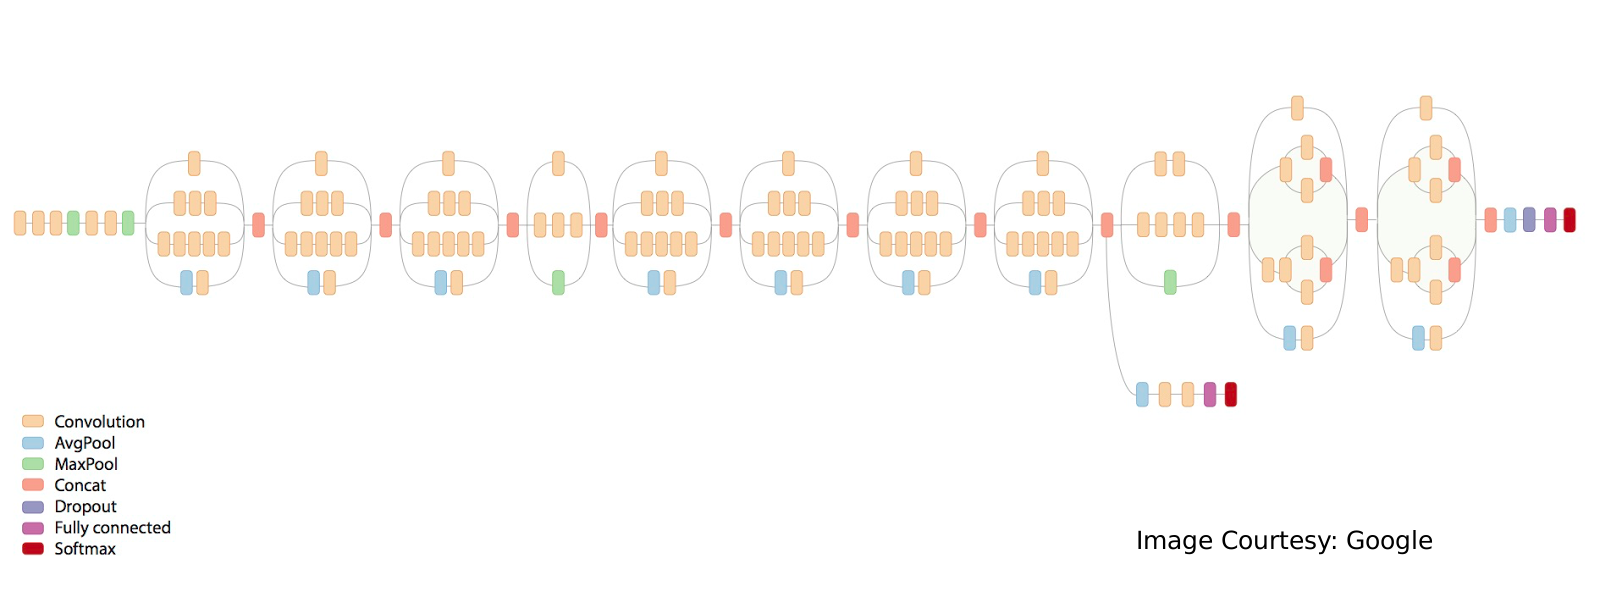
\includegraphics[scale=0.192]{inceptionrenamed.png}
\end{frame}

\section{Transfer Values}
\begin{frame}{Transfer Values}
	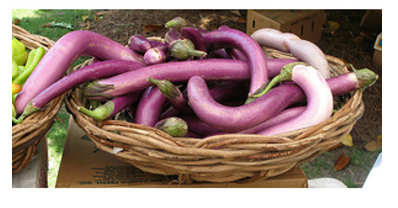
\includegraphics[scale=0.7]{brinjal1.png} \\
	\centering
	Brinjal 300px x 300px
\end{frame}


\begin{frame}{Transfer Values}
	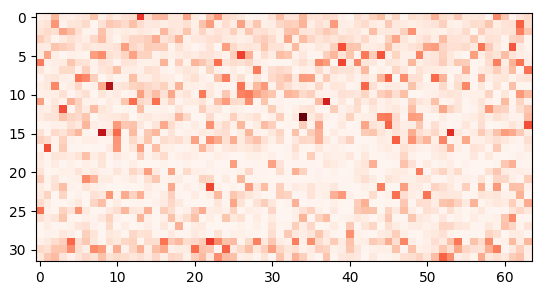
\includegraphics[scale=0.5]{brinjaltransfer1.png} \\
	\centering
	Transfer Values of above plotted image.
\end{frame}


\begin{frame}{Transfer Values}
	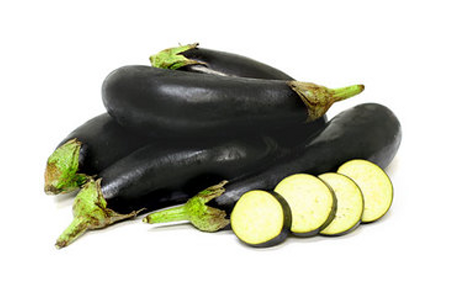
\includegraphics[scale=0.6]{brinjal2.png} \\
	\centering
	Brinjal 300px x 300px
\end{frame}


\begin{frame}{Transfer Values}
	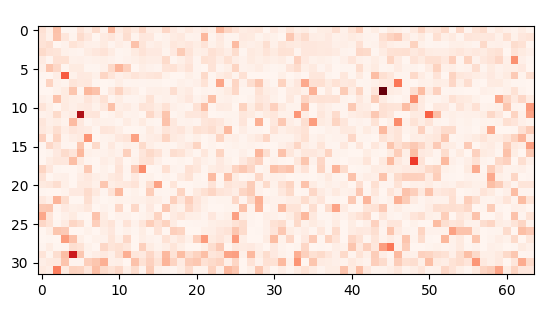
\includegraphics[scale=0.5]{brinjal2transfer.png} \\
	\centering
	Transfer Values of above plotted image.
\end{frame}


\begin{frame}{Transfer Values}
	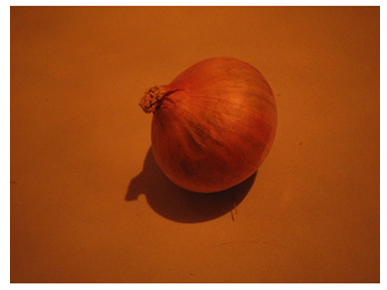
\includegraphics[scale=0.65]{onion1.png} \\
	\centering
	Onion 300px x 300px
\end{frame}


\begin{frame}{Transfer Values}
	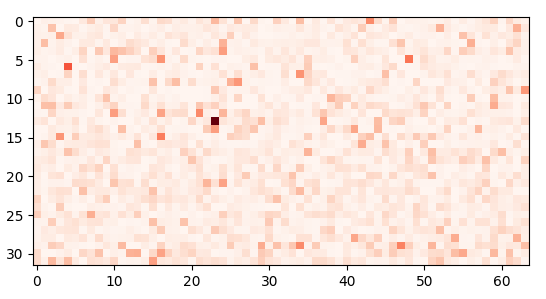
\includegraphics[scale=0.5]{onion1trans.png} \\
	\centering
	Transfer Values of above plotted image.
\end{frame}


\begin{frame}{Transfer Values}
	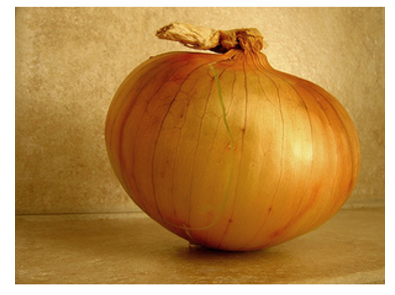
\includegraphics[scale=0.7]{onion2.png} \\
	\centering
	Onion 300px x 300px
\end{frame}


\begin{frame}{Transfer Values}
	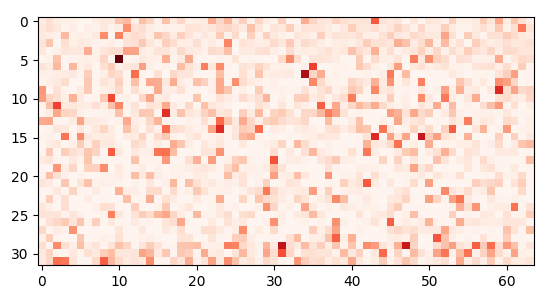
\includegraphics[scale=0.5]{onion2transfer.png} \\
	\centering
	Transfer Values of above plotted image.
\end{frame}

\section{t-SNE}
\begin{frame}{t-Distributed Stochastic Neighbor Embedding (t-SNE)}
	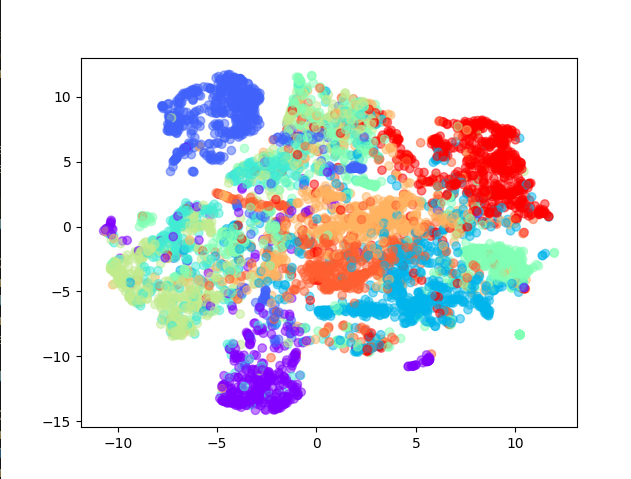
\includegraphics[scale=0.45]{TSNE.png}
\end{frame}

\section{Accuracy}
\begin{frame}{Accuracy}
	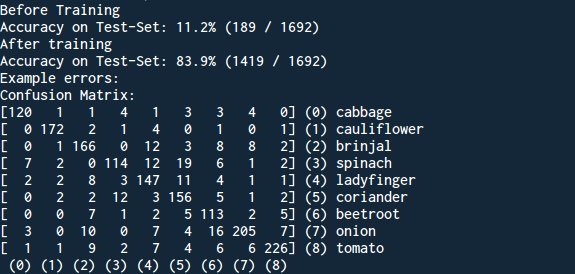
\includegraphics[scale=0.7]{confmatrix.png}
\end{frame}

\section{Example errors}
\begin{frame}{Example errors}
	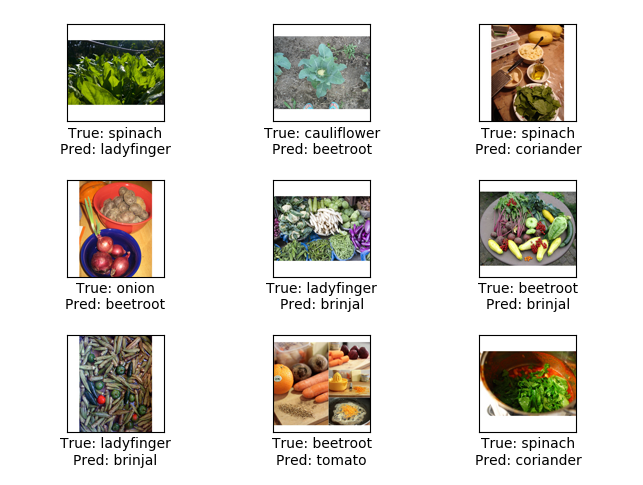
\includegraphics[scale=0.45]{exampleerrors.png}
\end{frame}

\section{Challenges Faced}
\begin{frame}{Challenges Faced}
	\begin{itemize}
		\item Not enough relevant data.
		\item Lack of memory for training Convolutional Neural Network from scratch.
		\item Classifying vegetables with similar features.
	\end{itemize}
\end{frame}

\section{Future Plans}
\begin{frame}{Future Plans}
% Please add the following required packages to your document preamble:
% \usepackage{graphicx}
\begin{table}[]
	\centering
	\label{my-label}
	\resizebox{\textwidth}{!}{%
		\begin{tabular}{|l|l|l|}
			\hline
			Sr. No & Work to be done & \begin{tabular}[c]{@{}l@{}}No. of days \\ required(approx.)\end{tabular} \\ \hline
			1 & Integrate this module with the logging system. & 5 \\ \hline
			2 & \begin{tabular}[c]{@{}l@{}}Train a Conv-Net from scratch and \\ try to achieve reasonable accuracy.\end{tabular} & 10 \\ \hline
			3 & \begin{tabular}[c]{@{}l@{}}Add Image Processing to find count of vegetables \\ which are counted rather than weighed.\end{tabular} & 8 \\ \hline
			4 & Collect and classify data. & Parallel \\ \hline
		\end{tabular}%
	}
\end{table}
\end{frame}


\section{Thank You}
\begin{frame}{Thank You}
	\centering
	
\includegraphics[scale=0.32]{robotthank.png}
\end{frame}
\end{document}
